% So we make this "beamer" rather than document!

\documentclass[11pt]{beamer}
% For handout add ,handout after 11pt

\usetheme[sectionpage=none,numbering=none]{metropolis}           % Use metropolis theme
	% To do printouts, add ", handout"  after aspectratio.
\usepackage{booktabs}
\usepackage{graphicx}
\usepackage{color}

\title{Unifying Data Science}
\author{\small Nick Eubank}
\date{\vspace*{.3in} \date}


% This is the beginning of a real document!
\begin{document}


\begin{frame}[c]
\maketitle
\end{frame}

\begin{frame}[c]{}
  By the end of this class, you will be able to:
\begin{enumerate}
  \item Understand how data science tools relate to one another using a unified conceptual framework,
  \item Answer causal questions\\
  \emph{Does X cause Y?}
  \item Execute a data science project from conception to delivery
\end{enumerate}
\end{frame}

\begin{frame}[c]{How did Data Science become a thing?}

\begin{itemize}
	\pause \item Academic research is organized into silos:
	\pause
	\begin{itemize}
		\item Computer Science
		\item Statistics
		\item Economics
		\item Political Science
		\item Engineering
	\end{itemize}
\end{itemize}
\pause $\Rightarrow$ Development of new tools occurred \emph{within} each silo.
\end{frame}


\begin{frame}[c]{Where are we today?}
Very little cross-pollination across silos
\begin{itemize}
	\pause \item Lots of duplication of development.
	\pause \item Every silo has its own vocabulary.
	\pause \item Each silo has focused on the aspects most relevant to their applications. e.g.:
	\begin{itemize}
		\pause \item CS likes to classify things and make predictions, don't care how model works
		\item Social scientists like to make causal statements, don't care about predictive power
	\end{itemize}
\end{itemize}
\end{frame}

\begin{frame}[c]{Blind Men and the Elephant}
\pause 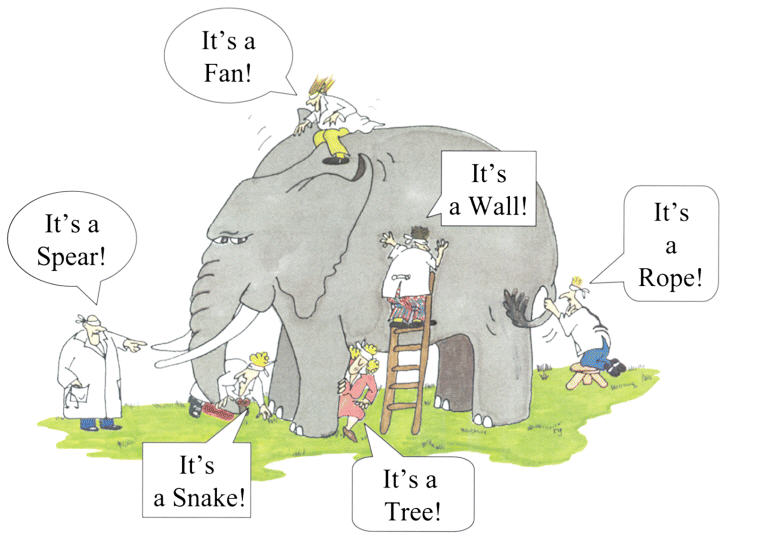
\includegraphics[width=\textwidth]{blindmenelephant.jpg}
\pause $\Rightarrow$ This is where data science is \emph{now.}
\end{frame}

\begin{frame}[c]{What do I think Data Science should be?}
\pause An effort to unify the development of quantitative methods \\
\pause $\rightarrow$ Recognize the elephant
\end{frame}

\begin{frame}[c]{This Class}
Discipline of learning how best to \alert{answer questions} using \alert{quantitative data.}
\end{frame}

\begin{frame}[c]{This Class}
\begin{enumerate}
  \item Introduce a taxonomy of questions \\
  {\color{gray} Descriptive, causal, predictive}
  \pause \item \alert{For each class of questions}, we will discuss:
  \begin{itemize}
    \item Intrinsic challenges to answering each class of questions
    \item What tools are best suited to each type of question
  \end{itemize}
\end{enumerate}
  \pause   By the end of the course, you should know when to reach for...
  \begin{itemize}
    \pause \item Unsupervised machine learning
    \item Supervised machine learning
    \item Range of causal inference techniques \\
    {\color{gray}e.g. experiments, matching, regression, differences-in-differences}
    \item Other approaches to descriptive analysis
  \end{itemize}
\end{frame}


\begin{frame}[c]{This Class}
The tool you use should be dictated by the question you seek to answer
\end{frame}

\begin{frame}[c]{This Class}
\begin{enumerate}
  \item Introduce taxonomy of questions\\
  \uncover<2->{{\color{gray}Practice generating questions}}
  \item Discuss descriptive questions \\
  \uncover<3->{{\color{gray}Relatively brief}}
  \item Learn causal inference \\
  \uncover<4->{{\color{gray}{ Deep dive -- $\sim$ half the semester}}}
  \item Discuss prediction \\
  \uncover<5->{{\color{gray}Relative merits of supervised machine learning v. causal methods}}
\end{enumerate}
\end{frame}

\begin{frame}[c]{Data Science Project}
Over semester, you will also develop a data science project from start-to-finish
\begin{itemize}
  \item Teams of 3-4, grouped by interest and experience
  \item On topic of your own choosing
\end{itemize}
\pause $\rightarrow$ Nice portfolio piece\\
\pause $\rightarrow$ MIDS first-years: Capstone with training wheels
\end{frame}

\begin{frame}[c]{Who Are We?}
  	I am a social scientist
  	\begin{itemize}
  		\pause \item PhD in Political Economy, Masters in Economics, BA in Economics and Political Science
      \item Research on international development, social networks, election administration, gerrymandering
  	\end{itemize}
    \vspace*{0.5cm}
    \pause Zeren Li (TA)
    \begin{itemize}
      \pause \item PhD Candidate in Political Science
       \item Studies Chinese politics
       \item Strong background in causal inference and machine learning
    \end{itemize}
\end{frame}

\begin{frame}[c]{Last Notes On This Class}
\begin{itemize}
  \pause \item First time this class has been taught \\
  (Familiar material; but new audience)
  \pause \item We'll do several evaluations over the semester of how things are going, and adjust as we go.
  \pause \item First few weeks won't be full representative.
  \begin{itemize}
    \pause \item If you're deciding whether to take this class, I'd suggest buying \emph{Mostly Harmless Econometrics} and skimming a few chapters to get a sense of material we'll focus on for much of semester.
  \end{itemize}
\end{itemize}
\end{frame}

\begin{frame}[c]{}
Course site: \url{http://www.unifyingdatascience.org}

\end{frame}


\end{document}
